\subsubsection{Kachelung und Normalisierung der Punktwolken}

Die vom GeoSN bereitgestellten LiDAR-Daten liegen in Kacheln von 2 km² vor. Zur Reduktion des Arbeitsspeicherbedarfs und zur Gewährleistung einer effizienten Rechenleistung, wurden diese Abschnitte mittels eines Splitting-Algorithmus in quadratische Unterkacheln mit einer Kantenlänge von 250 m segmentiert. Um das Zerschneiden von Baumkronen an Kachelbegrenzungen zu vermeiden, wurde ein Überlappungspuffer von 15 m definiert. Der nachfolgende Workflow erlaubt entweder die Prozessierung für einzelne Kachel-IDs oder eine automatisierte, sequenzielle Ausführung des gesamte Kachelsatzes. Diese modulare Partitionierung bietet zudem eine inhärente Datensicherheit gegen unvorhergesehene Programmabbrüche, da Zwischenergebnisse persistent gespeichert werden.

Im darauffolgenden Prozessschritt werden die topografischen Einflüsse durch eine Höhennormalisierung eliminiert. Da die originalen Z-Koordinaten der LiDAR-Punkte absolute Höhenwerte über der Normalhöhennull abbilden, überlagern sich die Objekthöhe und die Geländemorphologie. Für eine einheitliche vertikale Referenzierung müssen diese Werte in relative Höhen über dem Grund (Hight Above Ground, \ac{HAG}) überführt werden. Da der Datensatz bereits vorklassifiziert vorliegt, wird die Bodenklasse als Referenz verwendet. Mittels einer \textit{Delaunay-Triangulation} wird aus diesen Bodenpunkten ein kontinuierliches, nicht-überlappendes Dreiecksnetz als Digitales Geländemodell (\ac{DGM}) interpoliert. Die normalisierte HAG eines Punktes ergibt sich anschließend aus der Differenz zwischen seiner absoluten Z-Koordinate und der interpolierten Geländehöhe an der jeweiligen X-Y-Position. Mess- oder Interpolationsbedingte Artefakte, die zu negativen Höhenwerten führen, werden auf null gesetzt \cite{liIndividualTreeSegmentation2023}. Abbildung \ref{fig:norm} verdeutlicht die Verschiebung der Punktwolke an der Z-Achse verschoben, da die Bodenpunkte nun konsistent eine Höhe von Null aufweisen.
\begin{figure}[htbp]
    \centering
    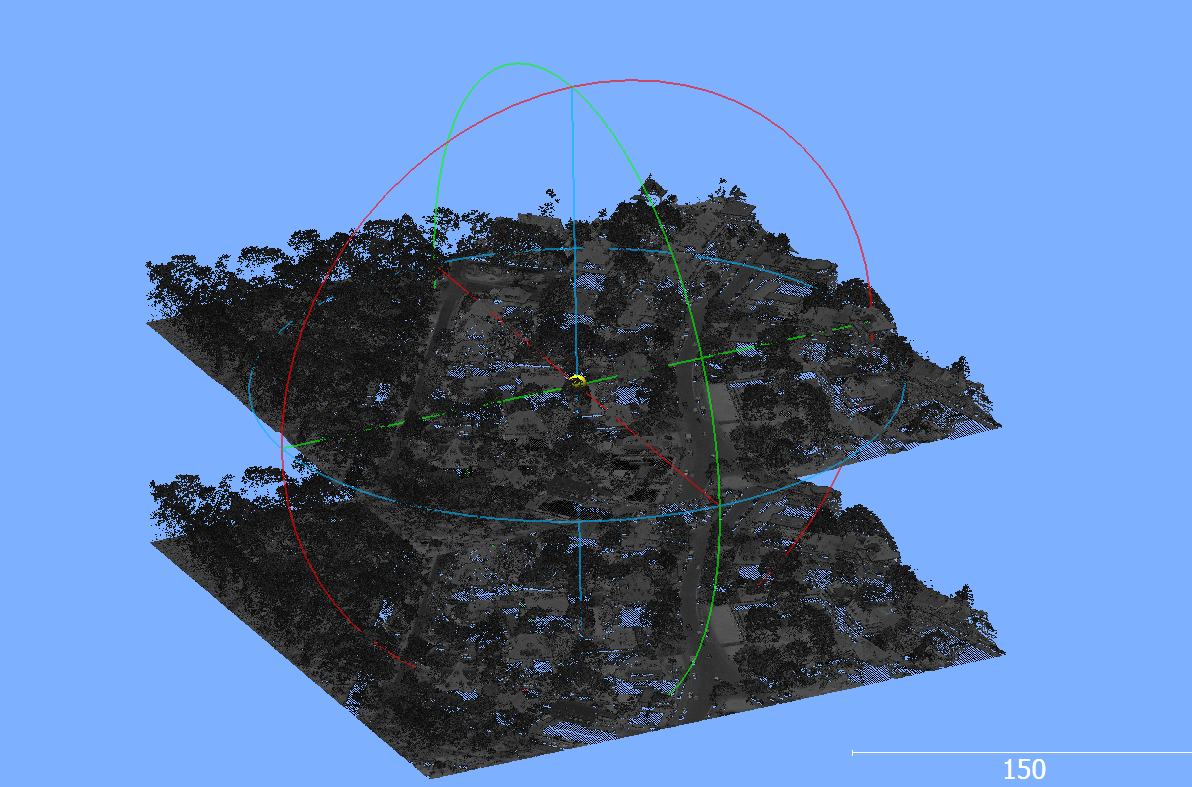
\includegraphics[width=0.63\columnwidth]{imgs/Normalisierung.png}
    \caption[Höhennormalisierung einer LiDAR-Punktwolke]{Höhennormalisierung einer LiDAR-Punktwolke mittels Delaunay-Triangulation in CloudCompare}\label{fig:norm}
\end{figure}

Die softwaretechnische Umsetzung dieses mathematischen Verfahrens wird durch folgende Pipeline in Code \ref{lst:pdal_normalize} realisiert.
\begin{lstlisting}[label={lst:pdal_normalize}, caption={[Normalisierungs-Pipeline]PDAL-Pipeline der Punktnormalisierung}, breaklines=true, breakatwhitespace=true]
pipeline_dict = [
    {"type": "readers.las", "filename": tile},
    {"type": "filters.hag_delaunay"},
    {"type": "filters.ferry","dimensions": "HeightAboveGround=>Z"},
    {"type": "filters.assign", "value": "Z=0 WHERE Z < 0"},
    {"type": "writers.las", "filename": output_path, "forward" : "all", "compression" : "true", "scale_z": "0.01"}
]
\end{lstlisting}
In der praktischen Umsetzung führt der Filter \textit{filters.hag\_delaunay} die beschriebene \textit{Delaunay-Triangulation} auf den Bodenpunkten durch, während \textit{filters.ferry} die berechnete relative Höhe in den primären Z-Kanal überträgt. Die Bereinigung der mathematischen Artefakten unterhalb des Bodens erfolgt schließlich über die Bedingung im \textit{filters.assign}-Operator. Nach Abschluss dieses Schritts, repräsentiert die Z-Koordinate jedes Punktes die relative Objekthöhe.
